\newpage

includes/Advanced/KarteUndMarkierungen/Operationsbefehl.tex
\subsubsection{Aufbau des Operationsbefehls}
\label{OPbef}
Fragestellung zur Planung des Operationsbefehls siehe auch:\ref{OPpla}

\begin{minipage}[t]{1\textwidth}
	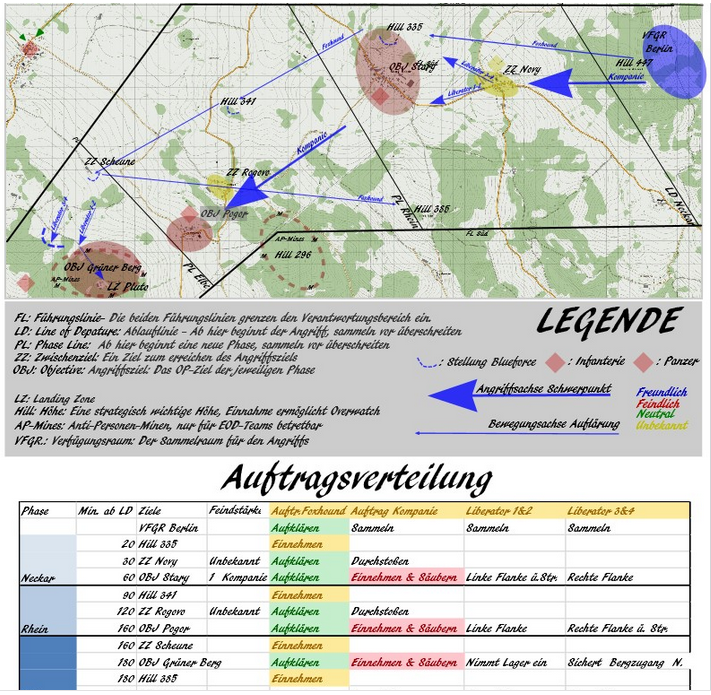
\includegraphics[width=\textwidth]{OP-Befehl.png}
\end{minipage}

\subsubsection{Linien}
\begin{longtable}{|p{3cm}|p{1,8 cm}|p{2,7cm}|p{4cm}|p{1,5cm}|} 																											\hline
	Linien				&		Abkürzung			&		Bezeichnung				&			Anmerkung 									&		Beispiel 			\\ \hline
	Führungslinie			&		FL				&		Angrenzende Himmelsrichtung	&			Die Führungslinien grenzen \newline den Verantwortungsbereich und \newline das Operationsgebiet ein. & FL Nord, FL SW \\ \hline
	Line of Depature (Ablauflinie)&		LD				&		Großer Fluss				&			Beim Überschreiten beginnt der Angriff und die Kampfhandlung 	&	LD Rhein, LD Donau			\\ \hline
	Phase Line (Kordinierungs-Führungslinie) & PL				&		Kleinere Flüsse			&			Eine OP unterteilt sich in zwei- drei räumlich und zeitlich getrennte Phasen, markiert durch die Phasenlinien	& PL Neckar, PL Inn, PL Isar	\\ \hline
	Sicherungslinie 		&		SL 				&		Insel					&			Sicherungslinien, auf denen der Feind abzuwehren ist.		&	SL Rügen, SL Sylt			\\ \hline
\end{longtable}

\subsubsection{Räume}
\begin{longtable}{|p{3cm}|p{1,8 cm}|p{2,7cm}|p{4cm}|p{1,5cm}|} 																											\hline
	Räume			&		Abkürzung			&		Bezeichnung				&			Anmerkung 									&		Beispiel 			\\ \hline
	Casualty Collection Point (Verwundeten Sammelstelle) & CCP	& 		Verwundeten- sammelstelle mit VS und Geländebeschreibung versehen & Hier werden die Verwundeten gesammelt		& 		CCP Ruine, CCP Abdera	\\ \hline
	Verfügungsräume		&		VGR				&		Bundesländer, Bundesstaaten	&			Sammelraum pro Phase, der als Sicher gilt. Häufig gibt es nur einen VGR vor der LD. 	&	VGR Bayern, VGR Pfalz \\ \hline
	Brückenkopf			&		BR				&		Helden				&			Wassernahe Stellung/Anlandungszone  im feindlichen Gebiet (Brücke, Strand, Flussseite)	& BR Herakles, BR Odin, BR Thor \\ \hline
\end{longtable}

\subsubsection{Ziele und Topographie}
\begin{longtable}{|p{3cm}|p{1,8 cm}|p{2,7cm}|p{4cm}|p{1,5cm}|} 																											\hline
	Ziele und Topographie	&		Abkürzung			&		Bezeichnung				&			Anmerkung 									&		Beispiel 			\\ \hline
	Zwischenziel			&		ZZ				&		Eingekürzter Name des Ortes oder konkrete Beschreibung des Ziels	&	Zwischenziele sind optionale Ziele, je nach Schlachtverlauf zu erreichen. ZZ mit Nummer versehen!	& ZZ Lager \#1, ZZ Novograd \#1 \\ \hline
	Objective			&		OBJ				&		Eingekürzter Name des Ortes oder konkrete Beschreibung des Ziels	&	Die Hauptziele der Operation		&		OBJ Abdera, OBJ Airport	\\ \hline
	Hill (Hügel/Anhöhe)		&		Hill				&		Hügel immer mit aktueller Höhenangabe versehen.	&	Stratgisch wichtige Anhöhen					&		Hill 136			\\ \hline
	Geländemarke		&		GM				&		Beschreibung, Ein, maximal zwei Wörter (Adjektiv, Subjekt)	&	Besondere Geländeeigenschaften werden beschrieben.	& 	GM Kugelbaum, GM tiefe Senke \\ \hline
\end{longtable}

\subsubsection{Zonen Luftwaffe und Logistik}
\begin{longtable}{|p{3cm}|p{1,8 cm}|p{2,7cm}|p{4cm}|p{1,5cm}|} 																											\hline
	Zonen Luftwaffe/Logistik	&		Abkürzung			&		Bezeichnung				&			Anmerkung 									&		Beispiel 			\\ \hline
	Landezone			&		LZ				&		Nato Alphabet			&			Landezone, die eingerichtet werden. Dabei handelt es sich ausdrücklich um Landezonen für Helikopter.	&	LZ Alfa, LZ Bravo 	\\ \hline
	Drop zone			&		DZ				&		NATO-Alphabet+ \#Nummer	&			Dropzone, Gebiet für das Abwerfen von Mensch (FJ) und Material per Fallschirm, bzw. Slingload Drops	&	DZ Alfa \#1		\\ \hline
	Pick up Zone			&		PZ				&		NATO-Alphabet+ \#Nummer	&			Zone zur Aufnahme von Mensch und Material, zum Ausfliegen oder Exfil per Boot				&	PZ Alfa \#1		\\ \hline
	Weapon Free Zone		&		WFZ				&		Codename, Einheitenname	&			Zone, in der eine Einheit Feuerfrei hat, wird per Codename von OPL freigegeben. (Hier OPL, Adler Freigabe für WFZ Heureka, bestätigen sie, kommen!)	& WFZ Heureka, Adler \\ \hline
	Bomben			&		Bomb				&		Codename, Einheitenname	&			Zone, die flächig gebombt werden soll - für Jabo, Jet-Einheiten							&	Bomb Hammerschlag, Condor \\ \hline
\end{longtable}

\subsubsection{Marsch}
\begin{longtable}{|p{3cm}|p{1,8 cm}|p{2,7cm}|p{4cm}|p{1,5cm}|} 																											\hline
	Marsch			&		Abkürzung			&		Bezeichnung				&			Anmerkung 									&		Beispiel 			\\ \hline
	Route, Anmarschweg	&		AW				&		Stadt / Routenname		&			Route des Feindes Oder der eigene Anmarschweg			&		AW Rom			\\ \hline
	Start Point (Start Punkt)	&		SP				&		Stadt / Routenname		&			Startpunkt des Marsches, ab hier beginnt der Marsch			&		SP Rom			\\ \hline
	Release Point (End Punkt)	&		RP				&		Stadt / Routenname		&			Endpunkt des Marsches, hier endet der Marsch mündet meist in ein VFGR	&	RP Rom			\\ \hline
	Check Point (Kontrollpunkt)	&	CP				&		Stadt / Routenname  + \#Nummer	&		Kontrollpunkt beim Marsch, hier wird bei passieren gemeldet, auf Befehl gehalten. &	CP Rom \#1		\\ \hline
	Passage Point (Durchlaufpunkt)	&	PP				&		Stadt / Routenname  + \#Nummer	&		Punkt zum Passieren, Meldung erforderlich!				&		PP Rom \#1	 		\\ \hline
	Technical Halt (Technischer Halt)) &	TH				&		Stadt / Routenname  + \#Nummer	&		Technischer Halt, zum Tanken, Munitionieren,Reperatur, etc.	&		TH Rom \#1			\\ \hline	
\end{longtable}